\documentclass[../../../main.tex]{subfiles}

\begin{document}

\begin{center}
	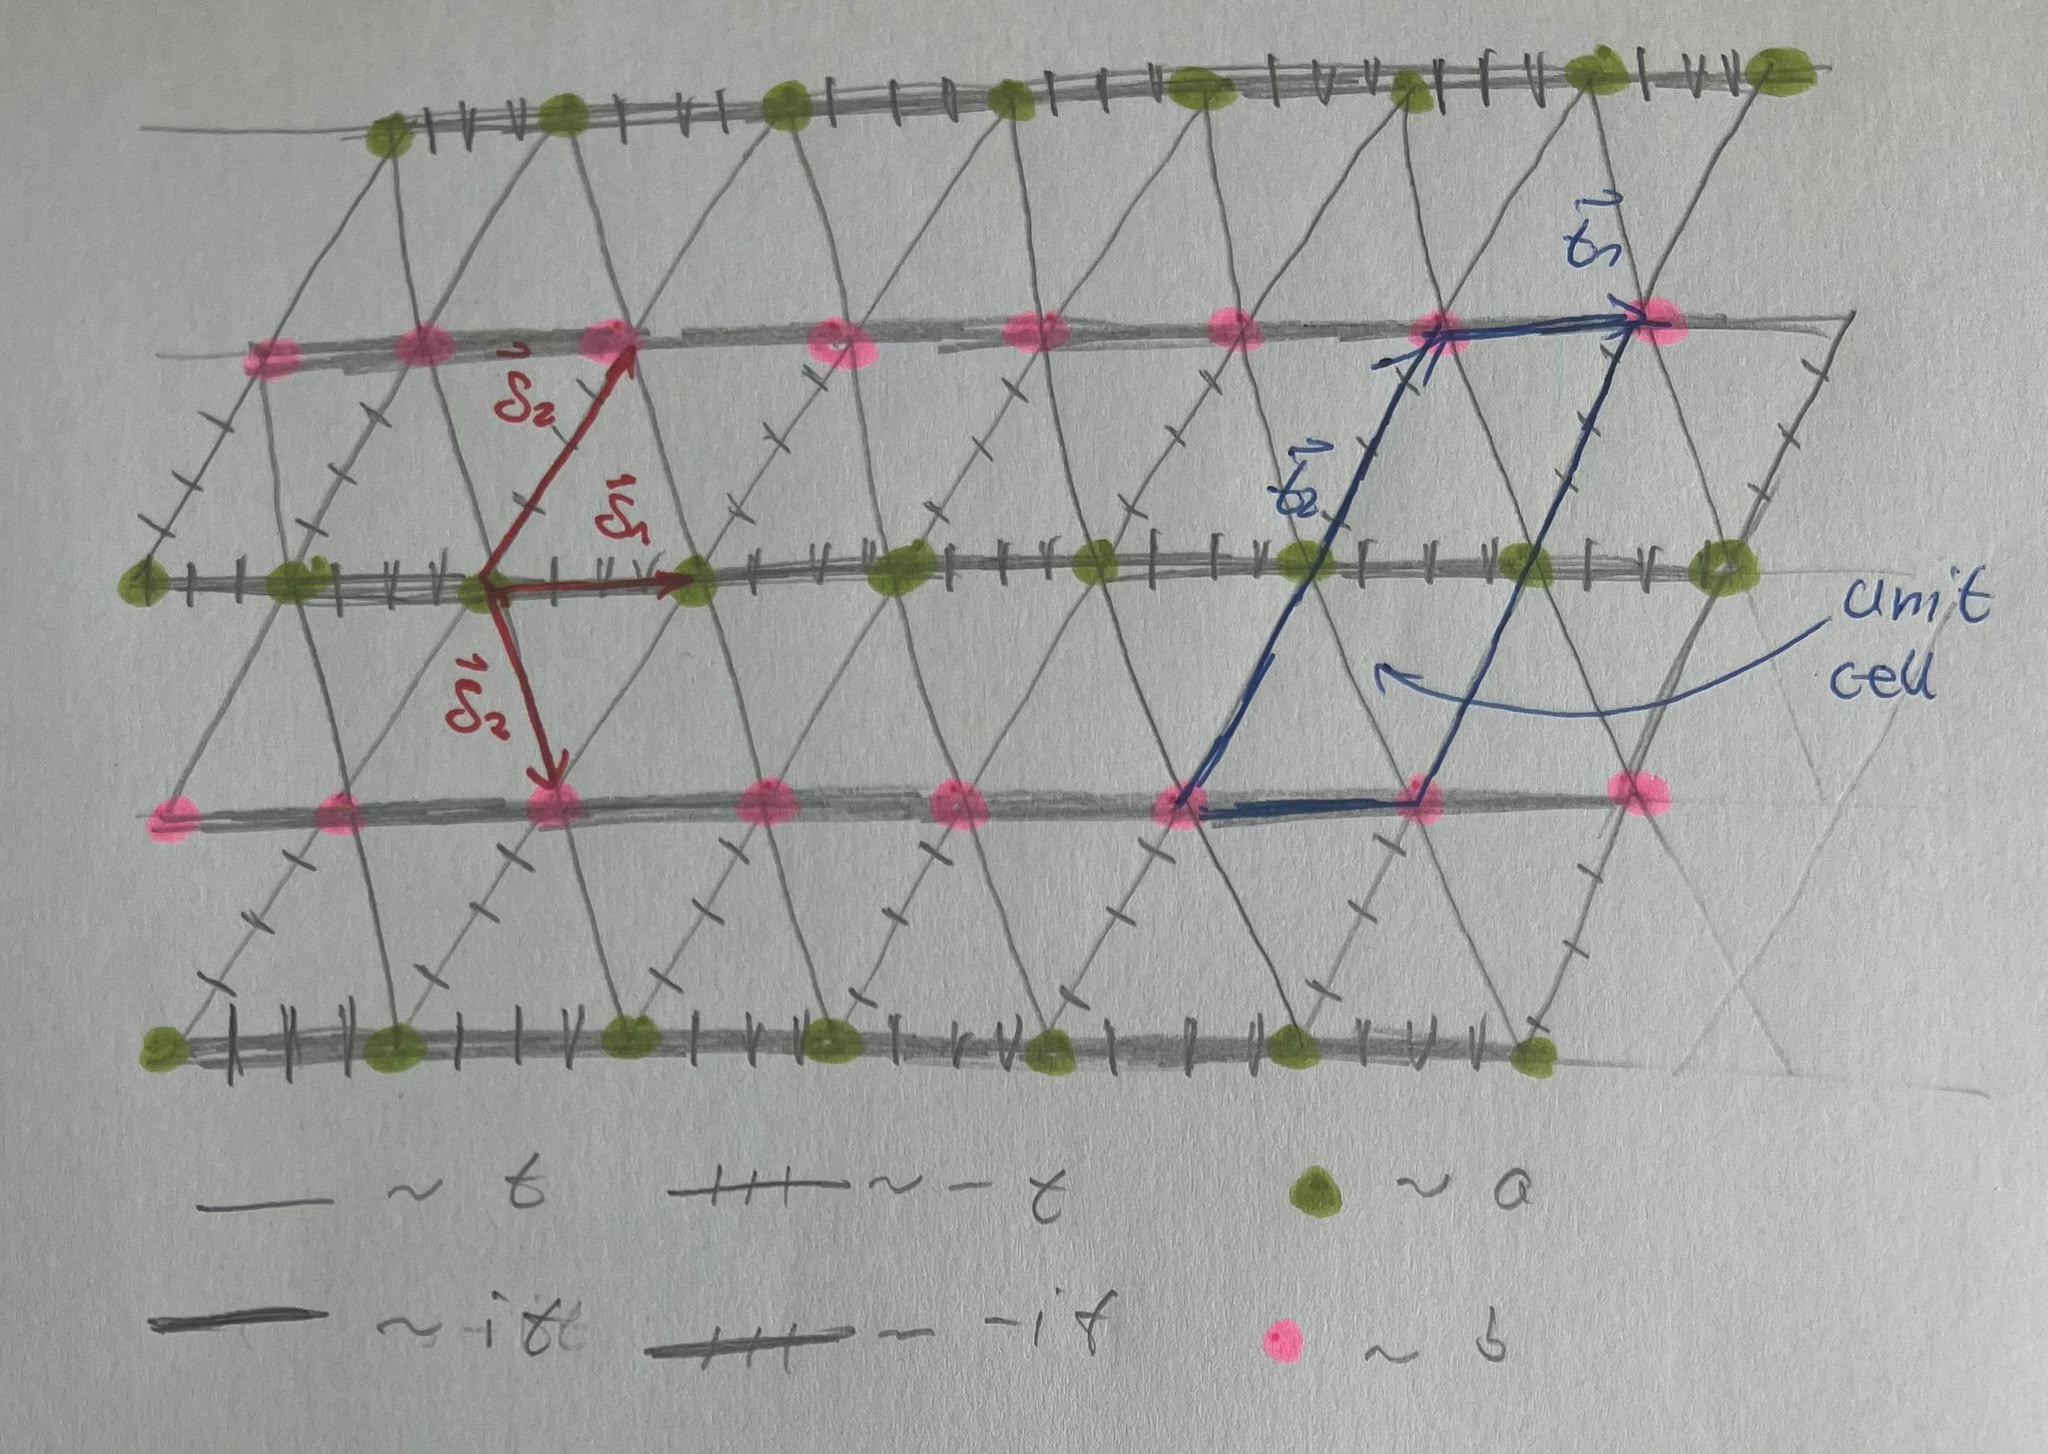
\includegraphics[width = \textwidth]{lattice-pi-half-flux-state.jpeg}
\end{center}

\subsubsection{Pedestrian Method}

This is very similar to the $\pi-0-$flux-state. The Bloch Hamiltonian in this case reads

\begin{equation}
H = 
\sum_{q,\sigma} 
\begin{pmatrix}
a_{q\sigma}^\dagger & b_{q\sigma}^\dagger 
\end{pmatrix}
\begin{pmatrix}
2t\sin(\vec{q}\vec{\delta}_1) + \mu_a&  2t\cos(\vec{q}\vec{\delta_3}) - 2it \sin(\vec{q}\vec{\delta}_2) \\
2t\cos(\vec{q}\vec{\delta}_3)  + 2it \sin(\vec{q} \vec{\delta}_2) & -2t\sin(\vec{q}\vec{\delta}_1) + \mu_b
\end{pmatrix}
\begin{pmatrix}
a_{q\sigma} \\
b_{q\sigma}
\end{pmatrix}
.
\end{equation}

So the only difference is $\cos\left( \vec{q} \vec{\delta}_1 \right) \rightarrow \sin\left(\vec{q}\vec{\delta}_1\right)$. Therefore, I will skip ahead in the calculations:

\textcolor{red}{Maybe I should show explicitly that $\mu = 0$, I guess $\mu_a = - \mu_b = \mu$ is clear} \textcolor{red}{I fucked up here again (bc I copied what was already wrong above). It is very lucky that this, though corresponding to a different unit cell than the shown in the cartoon, also gives a $\pi/2-\pi/2$-state.}

\begin{gather}
	\mu_a = \mu_b = 0, \\
	\varepsilon(\vec{k})_{\pm} = \pm 2|t|\sqrt{\sin^2(k_y) +\cos^2(k_y-k_x/2) + \sin^2(k_x/2)}
\end{gather}

\begin{equation}
\frac{1}{\sqrt{2\varepsilon_{+}(\varepsilon_+ + 2t\sin(k_y))}}
\begin{pmatrix}
\varepsilon_+ + 2t\sin(k_y) &-2t\cos(k_y - k_x/2) + 2ti\sin(k_x/2) \\
2t\cos(k_y-k_x/2) + 2ti\sin(k_x/2) &\varepsilon_+ + 2t\sin(k_y) 
\end{pmatrix}
\end{equation}


\begin{align}
	u_{11}u_{21} &= (t/\varepsilon_+)(\cos(k_y-k_x/2) + i \sin(k_x/2)) \\
	u_{11}^2 &= (1/2\varepsilon_+)(\varepsilon_+ + 2t\sin(k_y))
\end{align}


\begin{align}
	\frac12	\sum_\sigma\langle a_{i\sigma}^\dagger a_{i+\delta_1\sigma } \rangle &= \int\limits_{[-\pi,\pi]^2}  \frac{d^2k}{(2\pi)^2} e^{i k_y} \left[(1-2u_{11}^2)(1-f(\varepsilon_+)) + u_{11}^2\right] \\
	\frac12 \sum_\sigma \langle b_{i\sigma}^\dagger b_{i+\delta_1\sigma} \rangle &= \int\limits_{[-\pi,\pi]^2} \frac{d^2k}{(2\pi)^2} e^{i k_y} \left[(1-2u_{11}^2)f(\varepsilon_+) + u_{11}^2\right] \\
	\frac12 \sum_\sigma \langle a_{i\sigma}^\dagger b_{i+\delta_3\sigma} \rangle &= \int\limits_{[-\pi,\pi]^2} \frac{d^2k}{(2\pi)^2} e^{i(k_y-k_x/2)}u_{11}u_{21}(2f(\varepsilon_+) -1) \\
	\frac12 \sum_\sigma \langle a_{i\sigma}^\dagger b_{i+\delta_2\sigma} \rangle &= \int\limits_{[-\pi, \pi]^2} \frac{d^2k}{(2\pi)^2} e^{ik_x/2} u_{11}u_{21}^*(2f(\varepsilon_+)-1)
\end{align}

One has to be a bit careful of where the sign of $t$ enters when choosing $t=1$ for the self consistency. Due to the complex conjugation the $\sigma_z$-terms are insensitive to the sign of $t$, but the (real) $\sigma_x$- and $\sigma_y$-terms are not. The results (choosing $t=1$ are):

\begin{align}
	\frac12	\sum_\sigma\langle a_{i\sigma}^\dagger a_{i+\delta_1\sigma } \rangle &= -0.200169i\\
	\frac12	\sum_\sigma\langle a_{i\sigma}^\dagger a_{i-\delta_1\sigma } \rangle &= 0.200169i\\
	\frac12 \sum_\sigma \langle b_{i\sigma}^\dagger b_{i+\delta_1\sigma} \rangle &= 0.200169i\\
	\frac12 \sum_\sigma \langle b_{i\sigma}^\dagger b_{i-\delta_1\sigma} \rangle &= -0.200169i\\
	\frac12 \sum_\sigma \langle a_{i\sigma}^\dagger b_{i+\delta_3\sigma} \rangle &= 0.200169\\
	\frac12 \sum_\sigma \langle a_{i\sigma}^\dagger b_{i-\delta_3\sigma} \rangle &= 0.200169\\
	\frac12 \sum_\sigma \langle a_{i\sigma}^\dagger b_{i+\delta_2\sigma} \rangle &= 0.200169 \\
	\frac12 \sum_\sigma \langle a_{i\sigma}^\dagger b_{i-\delta_2\sigma} \rangle &= -0.200169
\end{align}

This complies with the cartoon on top. The value for $t$ is 

\begin{equation}
	|t_{ij}| = \left| J \langle \chi_{ij}\rangle^*(1+\kappa/2 - 4\kappa\abs{\langle \chi_{ij} \rangle}^2\right| \overset{\kappa = 10}{=} 0.88020 \, J. 
\end{equation}

The free energy is 

\begin{equation}
	\frac{\langle H \rangle}{N} = \int\limits_{[-\pi,\pi]^2}\frac{d^2k}{(2\pi)^2} \varepsilon_+(\vec{k}) (2f(\varepsilon_+(\vec{k}))-1) + 6\left( \tilde{J}\left(1-6\tilde{\kappa}\abs{\langle\chi_{i,i+\delta}\rangle}^2\right)\abs{\langle\chi_{i,i+\delta}\rangle}^2\right)
\ = -1.24978 \; J 
\end{equation}

\subsubsection{Pedro's Method}
The expression for the free energy is identical to the $0-\pi$-state except that $\gamma$ gets replaced by a different constant $\alpha$:

\begin{equation}
	\alpha = \int\limits_{[-\pi,\pi]^2} \frac{d^2k}{(2\pi)^2} \sqrt{\sin^2(k_y) + \cos^2(k_y-k_x/2) + \sin^2(k_x/2)} \approx 1.20102
\end{equation}

Crucally $\alpha$ is larger than gamma. The results for this method are

\begin{equation}
	\abs{\chi} = \alpha/6  = 0.20017,
\end{equation}


\begin{equation}
f_0 =\tilde{J} \left(\frac{1}{4\tilde{\kappa}} - \frac{2\alpha}{9} \sqrt{\frac{3}{\tilde{\kappa}}}\right) = -1.24979 \, J
\end{equation}

The methods agree.

\subsubsection{Chern number}

Here I will calculate the Chern number associated with the state. The relevant formula for a 2-band system is is 

\begin{equation}\label{Chernform}
	C = \frac{1}{4\pi} \int\limits_{\text{1.BZ}} d^2q \, \hat{h} \cdot \left(\partial_{q_x} \hat{h} \times \partial_{q_y} \hat{h}\right),
\end{equation}

where $\hat{h}$ is the normalized Bloch vector (\textcolor{red}{is this the correct terminology?}).

\begin{equation}
	\vec{h} = 2t
	\begin{pmatrix}
		\cos\left(\frac12(q_x - \sqrt{3}q_y)\right) \\
		\sin\left(\frac12(q_x + \sqrt{3}q_y)\right) \\
		\sin(q_x)
	\end{pmatrix} \equiv 2t
	\begin{pmatrix}
		\cos(\delta_3) \\
		\sin(\delta_2) \\
		\sin(\delta_1)
	\end{pmatrix}, \quad \abs{\vec{h}} \equiv \varepsilon(\vec{q})
\end{equation}

\textcolor{red}{Noteice that this is different than the one given above, I will resolve this at another time} I first simplify \ref{Chernform} a bit using

\begin{equation}
	\partial_\alpha \hat{h} = \frac{1}{\abs{\vec{h}}}\left(\partial_\alpha\vec{h} - \hat{h}\cdot\left(\partial_\alpha \vec{h}\right)\hat{h}\right).
\end{equation}

When applying this to \ref{Chernform}, 3 out of the for terms that appear are proportional to $\hat{h} \times \hat{h} = \vec{0}$.

\begin{equation}
	\Rightarrow C = \frac{1}{4\pi} \int\limits_{1.BZ}d^2q \, [\varepsilon(\vec{q})]^{-3} \vec{h} \cdot \left( \partial_{q_x}\vec{h} \times \partial_{q_y}\vec{h}\right)
\end{equation}

\begin{equation}
	\partial_{q_x}\vec{h} = t
	\begin{pmatrix}
		-\sin(\delta_3) \\
		\cos(\delta_2) \\
		2\cos(\delta_1)
	\end{pmatrix}, \qquad 
	\partial_{q_y}\vec{h} = \sqrt{3}t
	\begin{pmatrix}
		\sin(\delta_1) \\
		\cos(\delta_2) \\
		0
	\end{pmatrix}
\end{equation}

\end{document}
